\documentclass[UTF8]{report}
\usepackage[margin=0.5in]{geometry}
\usepackage{graphicx}
\usepackage{xetexko}

\title{%
    <컴퓨터프로그래밍 3> 실습 보고서 \\
    \large [제 10 주] 후위연산식계산기 1-2}
\author{201704150 허강준}
\date{\today}

\begin{document}
    \maketitle
    \tableofcontents

    \chapter{프로그램 설명서}
        본 보고서에서는 스택을 정의 및 구현하고 이를 응용하여 후위연산식을 계산하는 프로그램에 대해 기술한다.

        \section{프로그램의 전체 설계 구조 (MVC 등)}

            \paragraph{%
                \normalfont 본 스택 응용 프로그램은 크게 프로그램의 제어를 담당하는 Controller인 \texttt{app\_controller}, 입/출력을 담당하는 View인 \texttt{app\_view}, 그리고 스택을 정의하고 구현하는 \texttt{stack} 모델을 정의한다. \texttt{stack}모델은 이전에 계속 사용된 \texttt{vector} Type의 Wrapper 클래스이다. 여기에 더불어, 후위연산식 계산을 처리하기 위한 \texttt{postfix} Type을 추가로 정의한다.
            }

        \section{함수 설명서}

            \paragraph{\texttt{VECTOR(type)}}
            \paragraph{%
                \normalfont C++의 Standard Template Library에 정의된 Container Template Type인 \texttt{vector}를 일부 구현하였다. 구현된 메서드는 \texttt{new},  \texttt{delete}, \texttt{at}, \texttt{front}, \texttt{back}, \texttt{data}, \texttt{empty}, \texttt{size}, \texttt{max\_size}, \texttt{clear}, \texttt{insert}, \texttt{erase}, \texttt{push\_back}, \texttt{pop\_back}, \texttt{swap} 이다.
            }

            \paragraph{\texttt{stack}}
            \paragraph{%
                \normalfont \texttt{VECTOR(char) 의 type alias}
            }



            \paragraph{\texttt{app\_controller\_create}}
            \paragraph{\texttt{app\_controller\_run}}
            \paragraph{\texttt{app\_controller\_exit}}
            \paragraph{\texttt{app\_controller\_get\_result}}
            \paragraph{\texttt{app\_controller\_delete}}
            \paragraph{%
                \normalfont \texttt{app\_controller} 주요 공개함수들로 프로그램의 제어에 관여한다.
            }


            \paragraph{\texttt{getchar\_direct}}
            \paragraph{\texttt{appview\_in\_char\_directly\_from\_keyboard}}
            \paragraph{%
                \normalfont 키보드로부터 직접 키 입력을 받아온다. Control Sequence가 아닌 경우 echo도 같이 수행한다.
            }

            \paragraph{\texttt{appview\_in\_postfix\_expression}}
            \paragraph{%
                \normalfont 후위표현식을 사용자로부터 입력받는다.
            }

            \paragraph{\texttt{get\_i18n\_errormsg\_db}}
            \paragraph{%
                \normalfont 지정한 로케일에 해당하는 메세지 데이터베이스를 불러온다.
            }

            \paragraph{\texttt{appview\_out\_postfix\_evaluation\_error\_message}}
            \paragraph{%
                \normalfont 지정한 로케일에 해당하는 오류 메세지를 출력한다.
            }

            \paragraph{\texttt{appview\_out\_error\_in\_expression}})
            \paragraph{%
                \normalfont 입력받은 후위표현식에 오류가 있다는 메세지를 출력한다.
            }

            \paragraph{\texttt{postfix\_new }}
            \paragraph{\texttt{postfix\_delete}}
            \paragraph{%
                \normalfont 생성자/소멸자
            }

            \paragraph{\texttt{postfix\_set\_expression}}
            \paragraph{%
                \normalfont 입력받은 표현식을 객체에 설정
            }

            \paragraph{\texttt{postfix\_evaluated\_value}}
            \paragraph{%
                \normalfont 식 계산 결과를 리턴
            }

            \paragraph{\texttt{postfix\_evaluate}}
            \paragraph{%
                \normalfont 표현식을 바탕으로 후위연산식 계산을 수행
            }

            \paragraph{\texttt{appview\_out\_top\_of\_stack}}
            \paragraph{\texttt{appview\_out\_bottom\_of\_stack}}
            \paragraph{%
                \normalfont 스택 전체 출력시 처음과 끝이 각각 bottom, top임을 출력한다.
            }

            \paragraph{\texttt{appview\_out\_element}}
            \paragraph{%
                \normalfont 지정된 요소 하나를 출력한다.
            }
            
            \paragraph{\texttt{appview\_out\_new\_line}}
            \paragraph{%
                \normalfont 화면상에서 개행한다.
            }

            \paragraph{\texttt{appview\_out\_starting\_message}}
            \paragraph{\texttt{appview\_out\_ending\_message}}
            \paragraph{%
                \normalfont 프로그램의 시작과 끝을 알리는 메세지를 출력한다.
            }

            \paragraph{\texttt{stack\_new}}
            \paragraph{\texttt{stack\_delete}}
            \paragraph{%
                \normalfont 스택 객체 생성 및 삭제 함수
            }

            \paragraph{\texttt{stack\_push}}
            \paragraph{\texttt{stack\_pop}}
            \paragraph{%
                \normalfont 스택의 push, pop 동작 구현
            }

            \paragraph{\texttt{stack\_peek}}
            \paragraph{\texttt{stack\_at}}
            \paragraph{%
                \normalfont 스택의 peek, at 동작 구현
            }

            \paragraph{\texttt{stack\_size}}
            \paragraph{%
                \normalfont 스택에 저장된 요소의 크기를 반환한다.
            }

            \paragraph{\texttt{stack\_full}}
            \paragraph{\texttt{stack\_empty}}
            \paragraph{%
                \normalfont 스택이 꽉 찼는지, 비었는지 여부를 반환한다.
            }

        \section{종합 설명서}

            \paragraph{%
                \normalfont 본 프로그램은 사용자로부터 후위연산식 문자열을 입력받아 스택을 이용하여 해당 식을 계산하도록 하고 있다. 사용자는 \$ 문자를 입력하여 계산을 마칠 수 있도록 하며, 만일 입력한 식에 문제가 있는 경우 프로그램은 해당 사항에 대해 안내한다.
            }


    \chapter{프로그램 장단점/특이점 분석}
            \section{국제화 처리}
            \paragraph{%
                \normalfont 제작한 소프트웨어를 다른 언어 문화권에 판매하게 될 경우 해당 언어에 대한 대응이 필수적으로 이루어진다. 이때 자국의 언어로 소스코드에 직접 메세지를 입력할 경우 해당 작업이 어려워진다. 따라서 메세지를 별도의 데이터베이스로 구성하고 언어별로 인덱싱 하면 더욱 편리하게 국제화 작업을 끝마칠 수 있다.
            }

            \section{오류처리의 중요성}
            \paragraph{%
                \normalfont 컴퓨터 시스템은 기본적으로 프로그램을 실행하던 도중 프로그래머가 별도로 처리하지 않는 복구할 수 없는 오류(예외)가 발생할 경우 해당 프로그램의 제어를 탈취 후 종료시킨다. 그러나 이는 UX 및 시스템의 가용성을 저해하며, 오류의 원인을 명확하게 파악하기 어렵게 된다. 따라서 프로그래머는 예외가 발생하여 프로그램이 종료될 수도 있는 상황들에 대해 적절하게 처리해줄 필요가 있다.
            }

            \section{휴대폰이 멈추는 이유 \& 휴대폰 제조사별 오류 처리}
            \paragraph{%
                \normalfont 휴대폰 제조사는 각각의 개발 철학에 맞게 자사의 기기를 설계한다. 따라서 오류 처리에 대한 철학도 다를 수 있으며, 이는 메모리 공간 부족이나 시스템 인터럽트 처리, 혹은 보안 문제를 수반하는 메모리 문제(Stack smashing, Buffer overflow) 등의 관점에서 많은 점이 다르게 된다. 따라서 이를 잘 핸들링하는 제조사의 경우 기기가 잘 죽지 않는다고 생각할 수 있으나 그렇지 않은 경우 기기의 가용성을 저해하여 제조사에 대한 평가가 낮아지는 결과를 초래한다.
            }

    \chapter{실행 결과 분석}
        \section{실행 결과}
        \paragraph{%
            \begin{figure}[!htb]
                \centering
                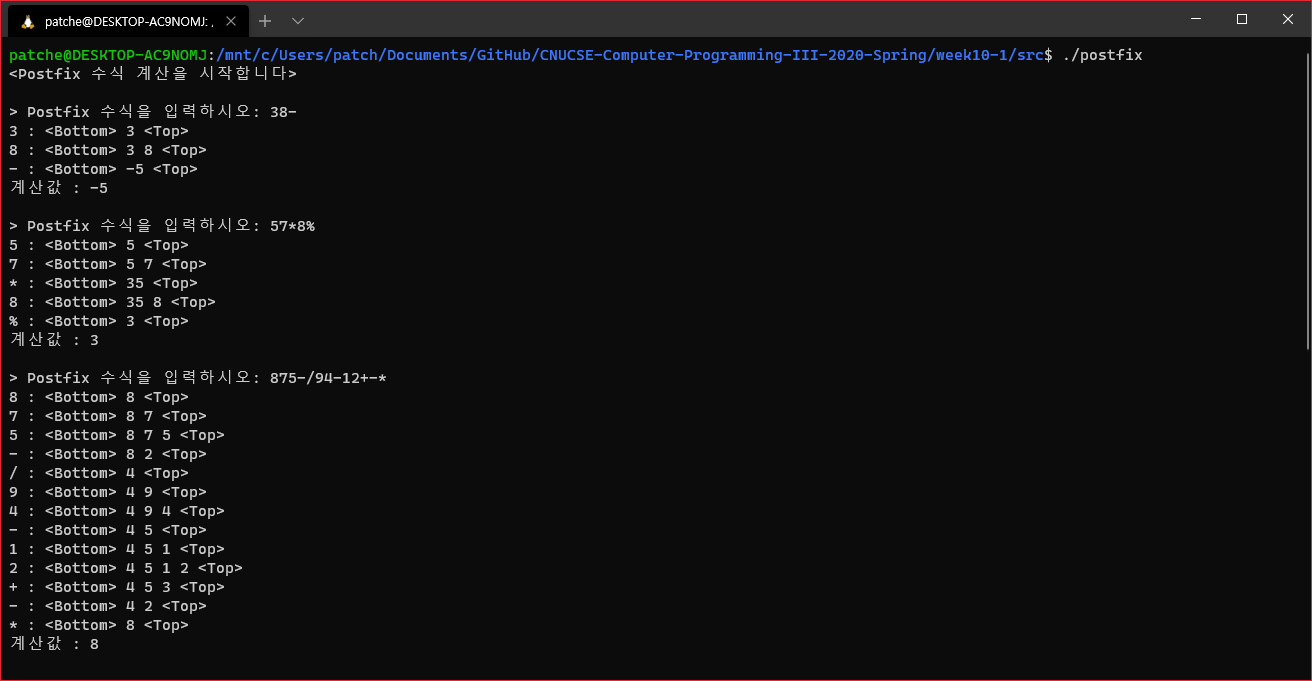
\includegraphics[width=\textwidth]{result_1.png}
                \caption{자료 제시 입력 실행결과 1}
                \label{}
            \end{figure}
            \begin{figure}[!htb]
                \centering
                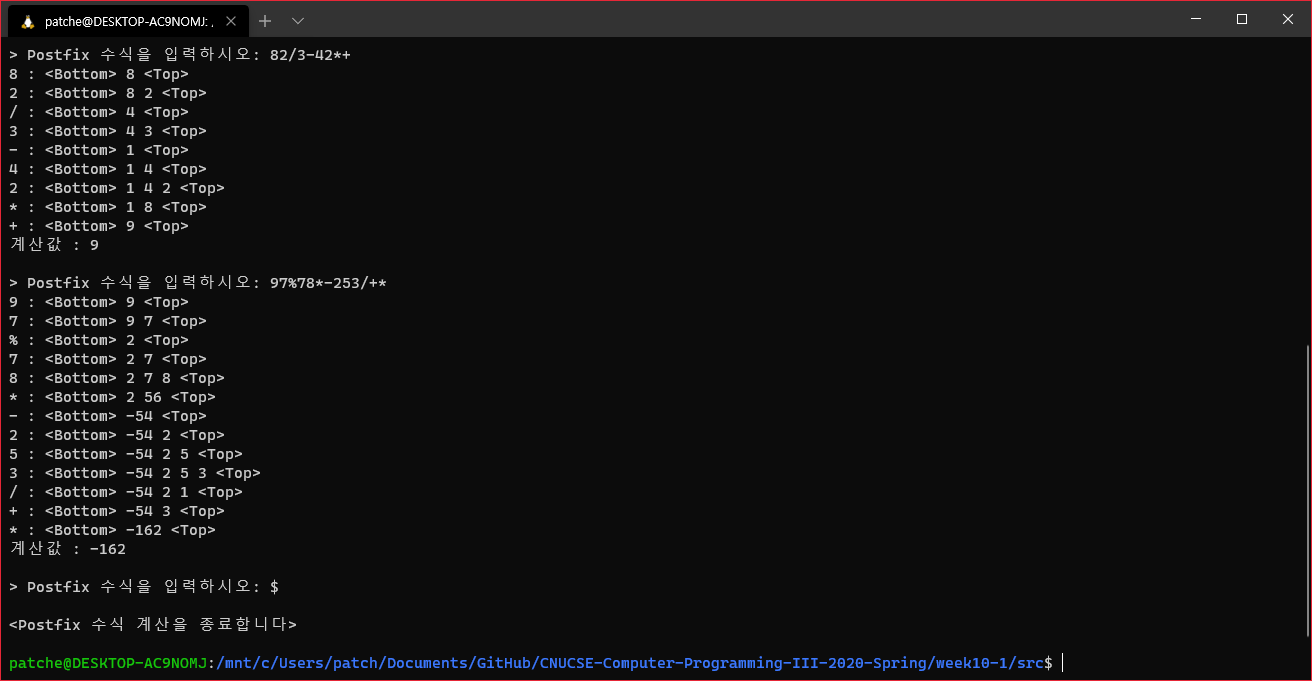
\includegraphics[width=\textwidth]{result_2.png}
                \caption{자료 제시 입력 실행결과 2}
                \label{}
            \end{figure}
            \begin{figure}[!htb]
                \centering
                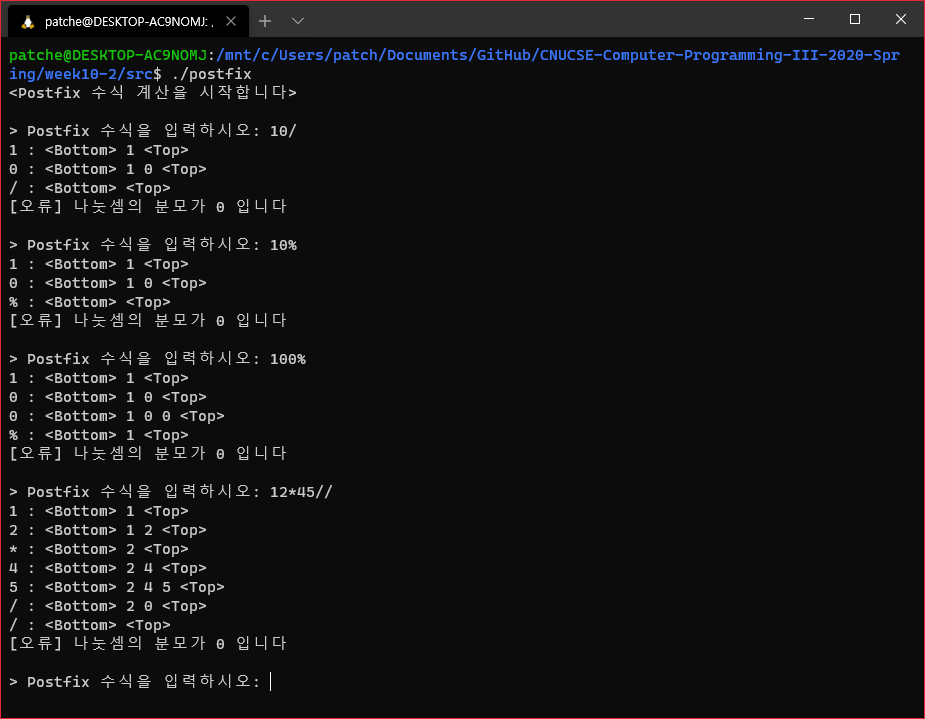
\includegraphics[width=\textwidth]{result_3.png}
                \caption{0으로 나누는 경우}
                \label{}
            \end{figure}
        }

        \newpage

        \section{입력과 출력}
            실습 자료에서 제시된 입력을 사용하였으며 출력 결과는 상기한 것과 같았음.
        \section{결과 분석}
            모든 입력에 대하여 정상적인 출력을 확인하였음.

    \chapter{소스코드}
        소스코드는 제출된 압축파일에 같이 동봉되어있으며 GitHub (0x00000FF/CNUCSE-Computer-Programming-III-2020-Spring) 에서도 열람할 수 있다.
\end{document}